\documentclass{beamer}
\usetheme{Antibes}
\usecolortheme{dolphin}

\setbeamertemplate{footline}[frame number]
\definecolor{g2}{RGB}{25, 0, 51}
\setbeamercolor{title}{fg=g2}
\setbeamercolor{frametitle}{fg=g2}
\usepackage[utf8]{inputenc}
\usepackage{amsmath}
\usepackage{amsfonts}
\usepackage{amssymb}
\usepackage{graphicx}
\usepackage{subcaption}

\institute{Department of Electronic Systems and Information Processing
 \\ Faculty of Electrical Engineering and Computing \\ University of Zagreb} 
\author{Iva Miholić \\ Advisor: Asst. Prof. Mile Šikić}
\title{ Bachelor Thesis No. 3743 \\ Information propagation in  online social networks}
\setbeamercovered{transparent} 
%\setbeamertemplate{navigation symbols}{} 
%\logo{} 
\date{9 Jul 2014}
%\subject{} 
\begin{document}

\begin{frame}
\titlepage
\end{frame}

%\begin{frame}
%\tableofcontents
%\end{frame}

\section{Introduction}
\subsection{Complex networks}
\begin{frame}
\frametitle{Networks}
\begin{figure}[htp]
\centering
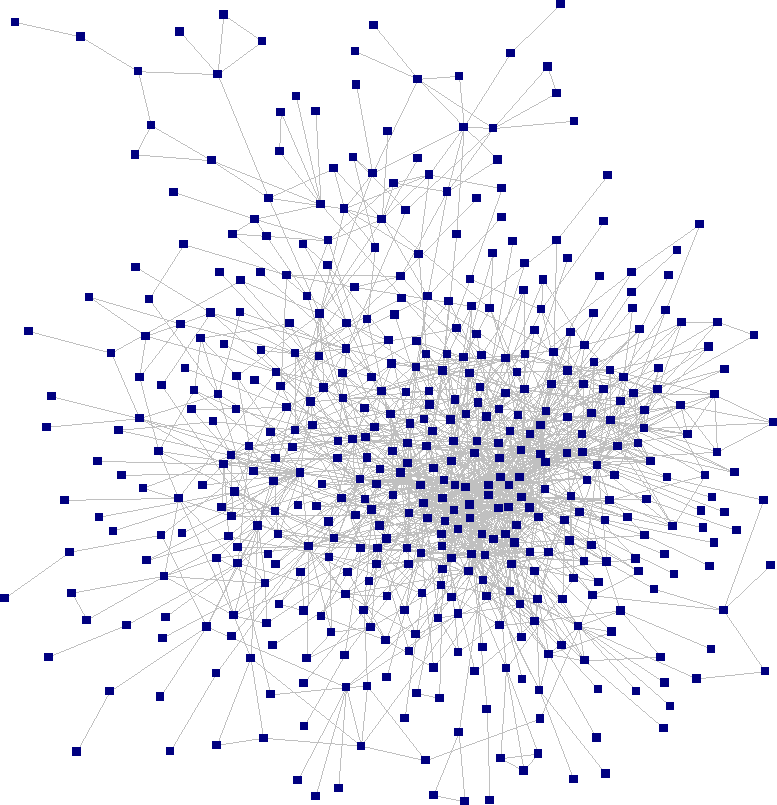
\includegraphics[scale=0.2]{figs/alters2.png}
\caption{A network graph of Paul Erd\~os and his collaborators. The nodes represent mathematicians and the edges represent the relationship "wrote a paper with".}
\label{net}
\end{figure}
\end{frame}

\begin{frame}
\begin{figure}[htp]
\centering
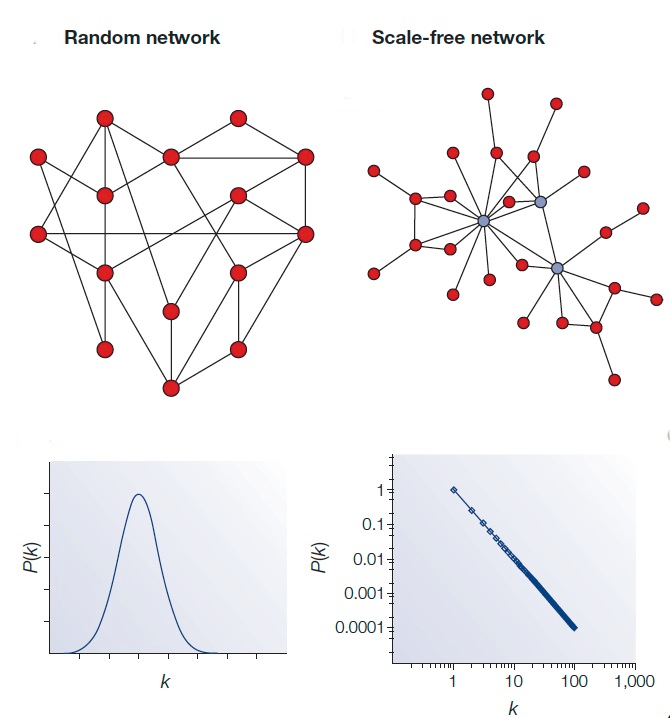
\includegraphics[width=0.7 \textheight]{figs/complex.jpg}
\caption{Comparison of a random and a scale-free network.  $p(k)$ stands for the probabilty that a vertex chosen unformly at random has degree $k$.}
\label{net}
\end{figure}
\end{frame}

\subsection{Information propagation}
\begin{frame}
\begin{itemize}
\item{propagation of the information item amongst the nodes of the social network}
\item{closed world $+$ social influence $=>$ information propagation similar to diffusion}
\item{In the real world, external influence is present. That is visible on the propagation dynamic.}
\item{Model of propagation that takes into account both internal and external influence.} 
\end{itemize}
\end{frame}

\section{Dataset}
\begin{frame}
\begin{figure}[htp]
\centering

\includegraphics[width=\textwidth]{figs/screenshot.png}
\caption{A screenshot of \emph{referendum2013.hr} site taken on 8 Jul 2014} 
\label{screenshot}
\end{figure}
\end{frame}

\begin{frame}
\frametitle{Registration dynamic}
\begin{itemize}
\item{$1.695$ million nodes, $4.461$ million edges}
\item{$11606$ registered users, $11$ recorded articles}
\end{itemize}
\begin{figure}[htp]
\centering
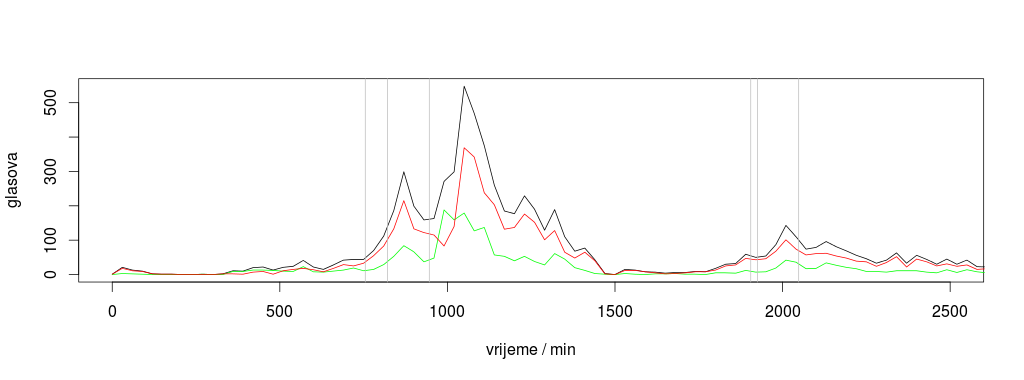
\includegraphics[scale=0.3]{figs/glas_ponuto.png}
\caption{Dynamic of registrations for the first two  days of application being active.}
%TODO  generiraj sliku
\label{glas_ponuto}
\end{figure}
\end{frame}

\begin{frame}
\frametitle{Datasets}
\begin{columns} 
\column{.5\textwidth}
Restricted Referendum Dataset
\begin{figure}
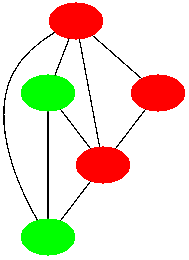
\includegraphics[scale=0.4]{figs/graphs1.png}
\end{figure} 
\column{.5\textwidth}
Complete Referendum Dataset
\begin{figure}
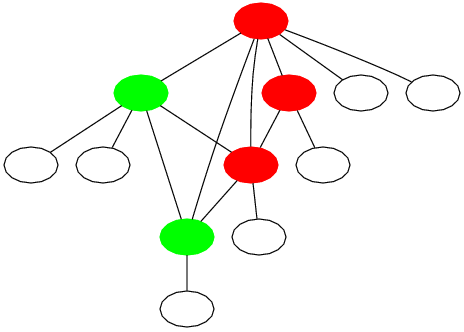
\includegraphics[scale=0.3]{figs/graphs2.png}    
\end{figure}
\end{columns}
\end{frame}

\begin{frame}
\begin{figure}[htp]
\centering
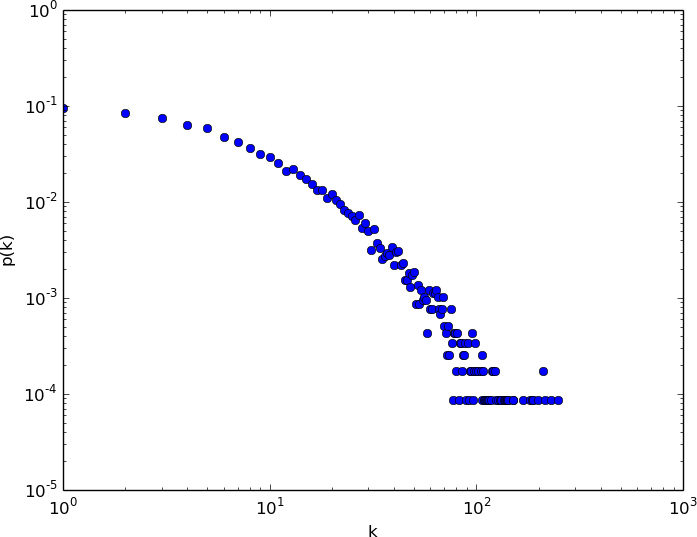
\includegraphics[scale=0.4]{figs/log_mali.png}
\caption{The degree distribution for the network of registered users. $p(k)$ stands for the probabilty that a vertex chosen unformly at random has degree $k$.} 
\label{glas_ponuto}
\end{figure}
\end{frame}

\begin{frame}
\begin{itemize}
\item{\bf{Q: Is the adoption of an information item for the given network mainly internal or external influence driven?}}
\item{information item = information on the existance of the application}
\item{network = Restricted and Complete Referendum Dataset}
\end{itemize}
\end{frame}

\section{Model}
\subsection{The proces of information propagation}

\subsection{The structure of the network}
\begin{frame}
\frametitle{The structure of the network}
\begin{itemize}
\item{nodes of social network + external nodes}
\item{every external node can influence every peer node (a node in social network)}
\item{set of external nodes form a complete graph}
\item{peer nodes do not influence the external nodes}
\end{itemize}
\end{frame}

\begin{frame}
\frametitle{Probability of activation}
\begin{equation}
\label{Pxy}
 P(x, y; \alpha, \beta, \gamma) = \frac{1}{1 + e ^ {-\alpha \ln(x + 1) - \beta \ln(y + 1) - \gamma}},	
\end{equation}

\begin{itemize}
\item{$x$ - the number of already active peer neighbours}
\item{$y$ - the number of already active authorities}
\item{$\alpha$ - \emph{peer coefficient}, measure of internal influence}
\item{$\beta$ - \emph{authority coefficient}, measure of external influence} 
\item{$\gamma$ - \emph{externality coefficient}, the impact of other factors}
\end{itemize}
\end{frame}

\begin{frame}
\frametitle{Assumptions}
\begin{itemize}
\item{Propagation happens in discrete time steps, from timestamp $1$ to timestamp $T$.}
\item{For every time stamp and every currently inactive node, success  of the node trying to become active is observed as a Bernoulli random variable.
}
\item{All observed events are independant.}
\item{From the time a node gets activated, its influence is constant and does not fade away with time. }
\item{Every external node has an equal probability of influencing any peer node.}
\end{itemize}
\end{frame}

\begin{frame}
\frametitle{Model estimation}
\begin{equation}
\label{Pxy}
 P(x, y; \alpha, \beta, \gamma) = \frac{1}{1 + e ^ {-\alpha \ln(x + 1) - \beta \ln(y + 1) - \gamma}},	
\end{equation}

\begin{itemize}
\item{Estimate parameters $\alpha$, $\beta$ and $\gamma$ with observed events of activation tryouts at every timestep for every currently unactive node using the principle of maximal likelihood.}
\end{itemize}
\begin{figure}[htp]
\centering
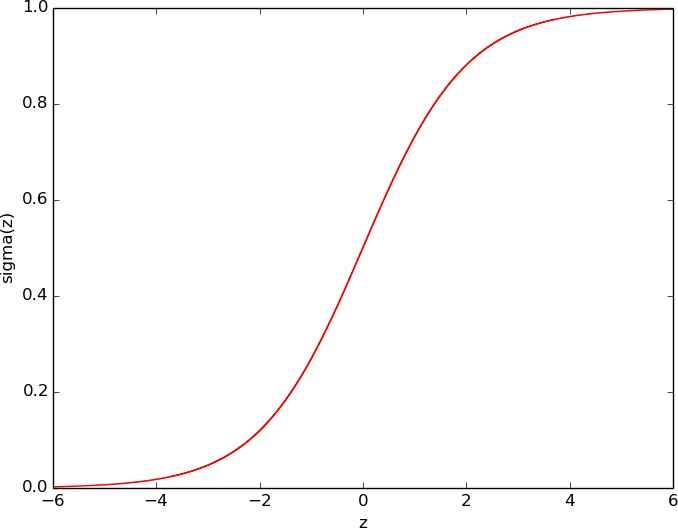
\includegraphics[scale=0.2]{figs/sig.png}
\caption{Function $\sigma(z) = \frac{1}{1 + e ^ {-z}}$.}
\label{sig}
\end{figure}
\end{frame}

\begin{frame}
\frametitle{Principle of maximal likelihood}
Take $\alpha$, $\beta$ and $\gamma$ that maximize 
\begin{equation}
\label{LF}
 L(\alpha, \beta, \gamma) = \prod_{x, y} P(x, y) ^ {A(x, y)} (1 - P(x, y)) ^ { N(x, y)}
\end{equation}
or minimize
\begin{equation}
\centering
 -\ln L(\alpha, \beta, \gamma) = -\sum_{x, y} A(x, y) \ln P(x, y) - \sum_{x, y} N(x, y) \ln (1 - P(x, y)). 
\end{equation}

\begin{itemize}
\item{$A(x,y)$ - number of observed succesful activations.}
\item{$N(x,y)$ - number of observed unsuccesful activations.}
\end{itemize}
\end{frame}

\begin{frame}
\frametitle{Randomization Test}
\begin{itemize}
\item{Given $\alpha$, $\beta$, $\gamma$ can we just conclude \\
$(\alpha >  \beta) => $ internal influence is dominant?}
\item{\emph{time-shuffle}  test is used to verify this conclusion.}
\end{itemize}
\textbf{\emph{time-shuffle} test}
\begin{itemize}
\item{randomize activation time of all eventually active nodes in the dataset}
\item{obtain $\alpha(D')$ and $\beta(D)'$ for the new dataset $D'$}
\item{update $S_\alpha$ and $S_\beta$}
\item{repeat}
\end{itemize}
\end{frame}    

\begin{frame}
\textbf{\emph{time-shuffle} test}
\begin{itemize}
\item{randomize activation time of all eventually active nodes in the dataset}
\item{obtain $\alpha(D')$ and $\beta(D)'$ for the new dataset $D'$}
\item{update $S_\alpha$ and $S_\beta$}
\item{repeat}
\end{itemize}
\vspace{1cm}
The \emph{strength of peer influence}, $S_\alpha$, is defined as
\begin{equation}
S_{\alpha} = P_{D' \in \mathcal{D}} (\alpha > \alpha(D')).
\end{equation}
and similarly for the \emph{strength of authority influence}, $S_\beta$:
\begin{equation}
S_{\beta} = P_{D' \in \mathcal{D}} (\beta > \beta(D')).
\end{equation}
\end{frame}

\section{Results}
\subsection{Restricted Referendum Dataset}
\begin{frame} 
\frametitle{Restricted Referendum Dataset}
$\alpha = 0.16432$,  $\beta = 0.41826$,  $\gamma = -8.84820$ \\
$S_\alpha = 0.996$, $S_\beta = 0.633$
\begin{figure}[htp]
\centering
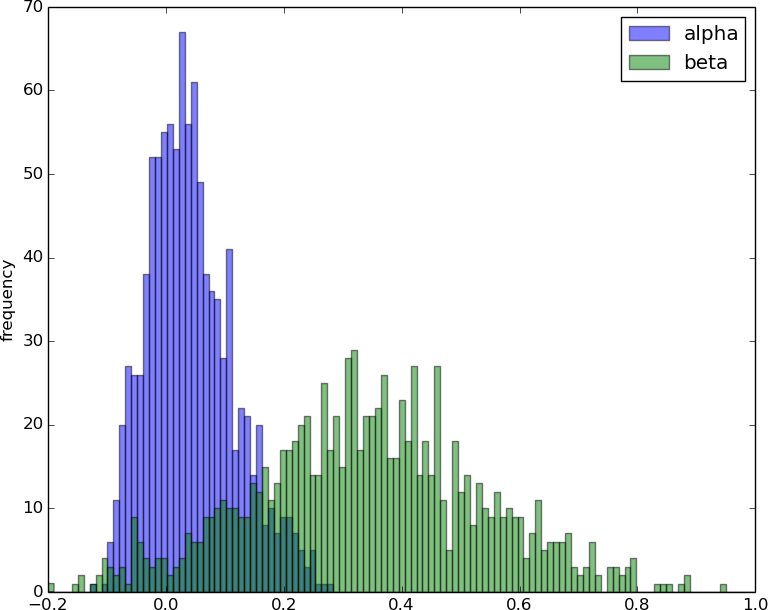
\includegraphics[scale=0.3]{figs/abg1000.png}	
\caption{Frequency histograms of estimated values of $\alpha$ (blue) and $\beta$ (green)  obtained for the Restricted Referendum Dataset with time-shuffle test based on $1000$ randomized instances.}
\label{hist_full}
\end{figure}
\end{frame}

\begin{frame}
\frametitle{Complete Referendum Dataset}
$\alpha = 1.44990$, $\beta = -1.02360$, $\gamma = -13.52627$ 
\begin{table}[htp]
\resizebox{\columnwidth}{!}{    
\centering
\begin{tabular}{|c|c|c|c|c|c|c|}
 \hline 
 \rule[-1ex]{0pt}{2.5ex} $y$ & $0$ & $1$ & $2$ & $3$ & $4$ & $5$  \\ 
 \hline 
 \rule[-1ex]{0pt}{2.5ex} successes & $0.77791$ & $9.00000$ & $7.34400$ & $3.91023$ & $4.52381$ & $3.74797$  \\ 
 \hline 
 \rule[-1ex]{0pt}{2.5ex} trials & $1697340$ & $1694519$ & $1693785$ & $1690362$ & $1689491$ & $1689169$ \\ 
 \hline 
 \rule[-1ex]{0pt}{2.5ex} success rate ($10 ^ {-6}$)& $0.458$ & $5.311$ & $4.336$ & $2.313$ & $2.678$ & $2.219$  \\ 
 \hline 
  \hline 
 \rule[-1ex]{0pt}{2.5ex} $y$ & $6$ & $7$ & $8$ & $9$ & $10$ & $11$ \\ 
 \hline 
 \rule[-1ex]{0pt}{2.5ex} successes & $ 1.26634$ & $0.89345$ & $0.67893$ & $1.41053$ & $3.40826$ & $1.62857$ \\ 
 \hline 
 \rule[-1ex]{0pt}{2.5ex} trials & $1687883$ & $1685728$ & $1684609$ & $1684391$ & $1684161$ & $1639898$ \\ 
 \hline 
 \rule[-1ex]{0pt}{2.5ex} success rate ($10 ^ {-6}$)& $0.750$ & $0.530$ & $0.403$ & $0.837$ & $2.024$ & $0.993$ \\ 
 \hline 
 \end{tabular}}
 \label{T2}
 \caption{Average frequencies of observed successful activations per time step, average frequencies of trials per time step  and success rates for the time period when $y$ authorities were active on the  Complete Referendum Datasets.}
\label{tab}
\end{table}
\end{frame}

\begin{frame}
\frametitle{Redefining  the model of external influence}
\begin{equation}
\label{Pxy}
 P(x, y; \alpha, \beta, \gamma) = \frac{1}{1 + e ^ {-\alpha \ln(x + 1) - \beta \ln(y + 1) - \gamma}},	
\end{equation}

\begin{itemize}
\item{$x$ - the number of already active peer neighbours}
\item{\textbf{$y$ - the number of activations of nodes with $0$ friends active at the time of the event}}
\vspace{1cm}
\item{now $y$ doesn't necessarily have positive correlation with time}
\end{itemize}
\end{frame}

\begin{frame}
\begin{columns}
\column{.5\textwidth}
\textbf{Restricted Referendum Dataset}\\
\begin{small}
$\alpha = 0.16697$, $\beta = 0.92495$, $\gamma = -8.60957$, $S_\alpha = 0.018$, $S_\beta = 0.959$ \\
- based on $1000$ randomized instances
\end{small}\begin{figure}[htp]
\centering
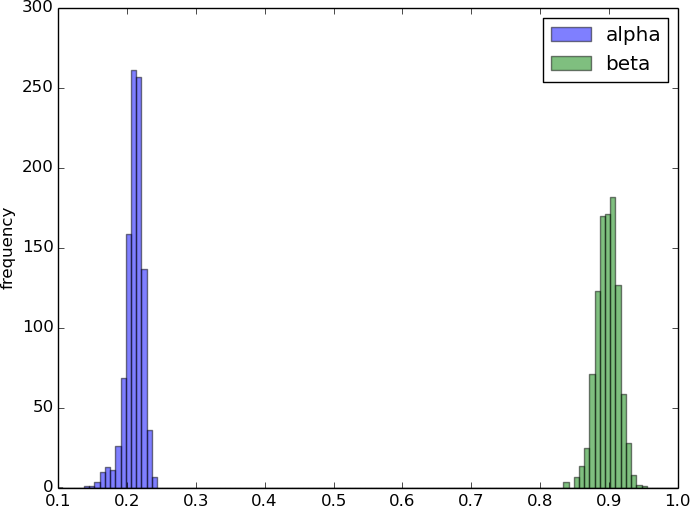
\includegraphics[scale=0.3]{figs/abg1000_2.png}	
\label{hist_full2}
\end{figure}
\column{.5\textwidth}
\textbf{Complete Referendum Dataset}\\
\begin{small}$\alpha = 0.89215$, $\beta = 1.36409$, $\gamma = -15.7230$, $S_\alpha = 1.000$, $S_\beta = 0.998$\\
- based on $500$ randomized instances \end{small}
\begin{figure}[htp]
\centering
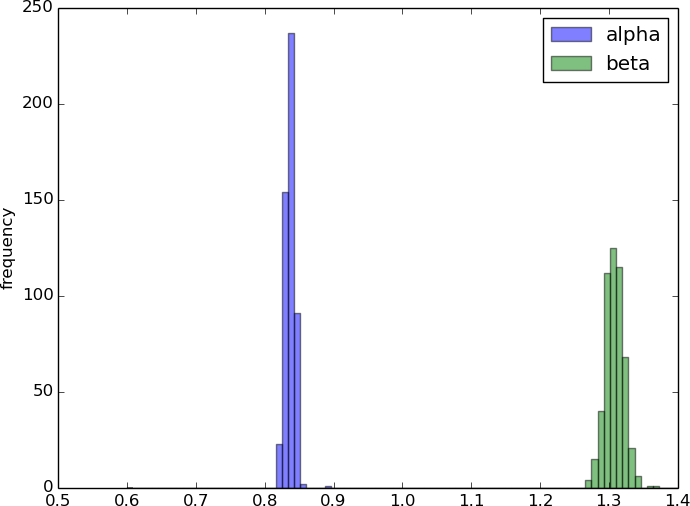
\includegraphics[scale=0.3]{figs/abg500v.png}	
\label{hist_full3}
\end{figure}
\end{columns}
\end{frame}

\begin{frame}
\begin{itemize}
\item{\bf{Q: Is the adoption of an information item for the given network mainly internal or external influence driven?}}
\item{\bf{A: The adoption is mainly external influence driven.}}
\end{itemize}
\end{frame}
\end{document}
